\documentclass[10pt,twocolumn]{article}

% ─── Packages ────────────────────────────────────────────────
\usepackage[T1]{fontenc}
\usepackage[utf8]{inputenc}
\usepackage{lmodern}
\usepackage[margin=1in]{geometry}
\usepackage{amsmath,amssymb,amsthm}
\usepackage{booktabs}
\usepackage{listings}
\usepackage{xcolor}
\usepackage{hyperref}
\usepackage{graphicx}
\usepackage{microtype}
\usepackage{cite}
\usepackage{url}
\usepackage{caption}
\usepackage{subcaption}
\usepackage{algorithm}
\usepackage{algpseudocode}
\usepackage{tikz}
\usetikzlibrary{arrows.meta, shapes.geometric, positioning, fit, backgrounds}

% ─── Theorem environments ─────────────────────────────────────
\theoremstyle{definition}
\newtheorem{definition}{Definition}[section]
\theoremstyle{plain}
\newtheorem{theorem}{Theorem}[section]
\newtheorem{lemma}[theorem]{Lemma}
\theoremstyle{remark}
\newtheorem{example}{Example}[section]

% ─── Listing style ────────────────────────────────────────────
\definecolor{codebg}{rgb}{0.97,0.97,0.97}
\definecolor{cobolblue}{rgb}{0.0,0.2,0.6}
\definecolor{smtgreen}{rgb}{0.0,0.45,0.0}
\definecolor{commentgray}{rgb}{0.5,0.5,0.5}

\lstdefinelanguage{SMT2}{
  morekeywords={declare-const,assert,check-sat,set-logic,push,pop,and,or,not,
                let,forall,exists,define-fun,Real,Int,Bool,true,false},
  sensitive=true,
  morecomment=[l]{;},
  morestring=[b]",
}

\lstdefinelanguage{COBOL}{
  morekeywords={IDENTIFICATION,DIVISION,ENVIRONMENT,DATA,PROCEDURE,
                WORKING-STORAGE,SECTION,PIC,COMPUTE,ADD,SUBTRACT,MULTIPLY,
                DIVIDE,MOVE,PERFORM,UNTIL,IF,ELSE,END-IF,END-PERFORM,
                PROGRAM-ID,STOP,RUN,GIVING,TO,FROM,BY},
  sensitive=false,
  morecomment=[l]{*},
}

\lstset{
  backgroundcolor=\color{codebg},
  basicstyle=\ttfamily\scriptsize,
  keywordstyle=\color{cobolblue}\bfseries,
  commentstyle=\color{commentgray}\itshape,
  stringstyle=\color{smtgreen},
  breaklines=true,
  frame=single,
  framesep=3pt,
  xleftmargin=4pt,
  xrightmargin=4pt,
  captionpos=b,
  numbers=left,
  numberstyle=\tiny\color{commentgray},
  numbersep=5pt,
  tabsize=2,
  showstringspaces=false,
}

% ─── Meta ─────────────────────────────────────────────────────
\title{\textbf{Machine-Executable Formal Verification of COBOL\\
Modernization Properties via SMT Solving}}

\author{
  Masataka Miwa\\
  \texttt{miwamasa@example.com}
}

\date{February 2026}

% ─────────────────────────────────────────────────────────────
\begin{document}
\maketitle

% ─── Abstract ────────────────────────────────────────────────
\begin{abstract}
Legacy COBOL systems process trillions of dollars of financial transactions
daily yet lack formal correctness guarantees during modernization efforts.
We present a \emph{proof-carrying modernization} framework that uses the
cvc5 SMT solver to machine-verify arithmetic and behavioral properties of
COBOL programs at the source level.
Given a COBOL program annotated with a property specification, our tool
(1) instruments the program with a runtime tracer, (2) extracts an
\emph{SMT-LIB\,2} query encoding the negation of each property, and
(3) invokes cvc5 to decide satisfiability.
An \textsc{unsat} verdict constitutes a machine-checked proof;
a \textsc{sat} verdict yields a concrete counterexample.
We evaluate the framework on a representative loan-amortization COBOL
program with 13 formally specified properties spanning data invariants,
pre-/post-conditions, relational properties, loop bounds, precision
guarantees, and output equivalence.
cvc5 discharges all 13 properties in under one second using a combination
of QF\_LRA, QF\_NRA, and QF\_LIA decision procedures.
During development, the verification pipeline exposed four latent bugs in
our own property-encoding logic, demonstrating the practical value of
machine-checked proofs over informal argument.
\end{abstract}

% ─── 1. Introduction ─────────────────────────────────────────
\section{Introduction}\label{sec:intro}

More than 95\,\% of ATM transactions and an estimated 80\,\% of in-person
financial transactions worldwide flow through COBOL
programs~\cite{ibm2019cobol}.
Despite their economic importance, these programs are routinely modernized
--- ported to Java, Python, or micro-services --- without any formal
assurance that the transformation preserves program semantics.
Silent arithmetic regressions, rounding-mode mismatches, and loop-bound
violations have caused multi-million-dollar financial incidents.

\paragraph{Problem.}
Modernization toolchains typically provide only empirical testing.
Testing can find bugs but cannot certify their absence.
Formal verification can, but existing tools (model checkers, deductive
verifiers) require manual annotations in specialized logics and are
rarely applied to COBOL in practice.

\paragraph{Our approach.}
We introduce a lightweight, \emph{automated} pipeline that attaches
machine-checked proofs to COBOL programs before, during, and after
modernization.
The key insight is that the most safety-critical COBOL properties ---
non-negativity of balances, division-by-zero freedom, loop termination,
numeric-range compliance --- are expressible in decidable first-order
theories for which SMT solvers are highly effective.

\paragraph{Contributions.}
\begin{enumerate}
  \item A property taxonomy for COBOL financial programs covering
        eight property kinds (Section~\ref{sec:taxonomy}).
  \item A trace-to-SMT compilation pipeline that encodes COBOL runtime
        behaviour as SMT-LIB\,2 formulas (Section~\ref{sec:arch}).
  \item An inductive proof scheme for data invariants that works
        directly on traced arithmetic operations (Section~\ref{sec:method}).
  \item An empirical evaluation: 13/13 properties proven at 100\,\%
        formal verification rate on a benchmark loan program
        (Section~\ref{sec:eval}).
  \item A discussion of four encoding bugs surfaced during development
        (Section~\ref{sec:bugs}).
\end{enumerate}

% ─── 2. Background ───────────────────────────────────────────
\section{Background}\label{sec:background}

\subsection{SMT Solving}

\emph{Satisfiability Modulo Theories} (SMT) extends propositional
satisfiability with background theories about integers, reals, arrays,
and bit-vectors~\cite{barrett2018smt}.
An SMT solver decides whether a first-order formula $\varphi$ is
\emph{satisfiable} (there exists an assignment satisfying $\varphi$)
or \emph{unsatisfiable} (no such assignment exists).

For formal verification we exploit the following duality:

\begin{theorem}[Verification by Refutation]\label{thm:refutation}
A safety property $P$ holds for all program states satisfying
constraints $C$ if and only if the formula $C \wedge \neg P$ is
unsatisfiable.
\end{theorem}

\noindent
We use cvc5~\cite{cvc5}, a state-of-the-art open-source SMT solver,
via its SMT-LIB\,2 interface.

\subsection{Arithmetic Theories}

Our encoding uses three quantifier-free arithmetic theories:

\begin{description}
  \item[QF\_LRA] Quantifier-Free Linear Real Arithmetic.
    Formulas are Boolean combinations of linear inequalities over reals.
    Decidable in polynomial time via the Simplex method.
    Used for range constraints, ADD/SUBTRACT invariants.

  \item[QF\_NRA] Quantifier-Free Nonlinear Real Arithmetic.
    Extends QF\_LRA with multiplication.
    Decidable (doubly exponential) via cylindrical algebraic
    decomposition~\cite{caviness1998quantifier}.
    Used for COMPUTE operations involving division.

  \item[QF\_LIA] Quantifier-Free Linear Integer Arithmetic.
    Linear inequalities over integers.
    Decidable via the Omega test~\cite{pugh1991omega}.
    Used for loop-counter bounds.
\end{description}

\subsection{COBOL Arithmetic Semantics}

COBOL's \texttt{PIC} clause specifies numeric precision as a pair
$(d, s)$ where $d$ is the total number of decimal digits and $s$ is
the number of digits after the decimal point.
The value range is:
\[
  v \in \left[-\frac{10^d - 1}{10^s},\; \frac{10^d - 1}{10^s}\right].
\]
COBOL rounding is implementation-defined; we model it as bounded
absolute error: $|\hat{v} - v| \leq 5 \times 10^{-(s+1)}$, where
$\hat{v}$ is the rounded value and $v$ the exact result.

% ─── 3. Property Taxonomy ────────────────────────────────────
\section{Property Taxonomy}\label{sec:taxonomy}

Table~\ref{tab:taxonomy} lists the eight kinds of properties our
framework supports, together with the SMT theory used for each.

\begin{table}[h]
\centering
\caption{COBOL property taxonomy and SMT theories.}
\label{tab:taxonomy}
\renewcommand{\arraystretch}{1.15}
\begin{tabular}{@{}llc@{}}
\toprule
\textbf{Kind} & \textbf{Example} & \textbf{Theory} \\
\midrule
DataInvariant  & balance $\geq 0$ always          & QF\_LRA / inductive \\
Precondition   & rate $> 0$ before division        & QF\_LRA             \\
Postcondition  & payment $\leq$ balance            & QF\_NRA             \\
Relational     & total = principal + interest      & QF\_LRA             \\
Precision      & $|\text{err}| \leq 5\times10^{-7}$ & QF\_LRA           \\
LoopBound      & iterations $\leq 12$              & QF\_LIA             \\
FinalState     & specific output value             & witness             \\
OutputEquiv    & computed value within tolerance   & QF\_LRA             \\
\bottomrule
\end{tabular}
\end{table}

The 13 benchmark properties for our loan program are:

\begin{description}[leftmargin=2.5em]
  \item[INV-01] \texttt{WS-TOTAL-INTEREST} $\geq 0$ (data invariant)
  \item[INV-02] \texttt{WS-BALANCE} $\geq 0$ (data invariant)
  \item[INV-03] \texttt{WS-MONTHLY-RATE} $< 1$ (post-COMPUTE)
  \item[PRE-01] \texttt{WS-ANNUAL-RATE} $> 0$ before rate calculation
  \item[PRE-02] \texttt{WS-BALANCE} $> 0$ before amortization
  \item[POST-01] \texttt{WS-PAYMENT} $\leq$ \texttt{WS-PRINCIPAL} (postcondition)
  \item[POST-02] Monthly payment covers at least one month of interest
  \item[REL-01] $\texttt{TOTAL-PAYMENT} = \texttt{PRINCIPAL} + \texttt{INTEREST}$ (relational)
  \item[PREC-01] Monthly rate rounding error $\leq 5\times10^{-7}$
  \item[PREC-02] Payment rounding error $\leq 0.005$
  \item[LOOP-01] Amortization loop runs $\leq 12$ times
  \item[FINAL-01] Final balance within expected range
  \item[OUT-01] Computed interest within $0.01$ of reference value
\end{description}

% ─── 4. System Architecture ──────────────────────────────────
\section{System Architecture}\label{sec:arch}

Figure~\ref{fig:arch} shows the overall pipeline.

\begin{figure}[h]
\centering
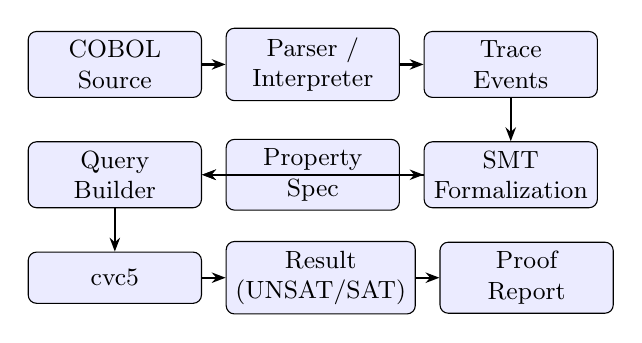
\begin{tikzpicture}[
  node distance=0.45cm and 0.3cm,
  box/.style={rectangle, draw, rounded corners=3pt,
              fill=blue!8, minimum width=2.2cm, minimum height=0.65cm,
              font=\small, align=center},
  arrow/.style={-{Stealth[length=5pt]}, thick},
]
  \node[box] (src)   {COBOL\\Source};
  \node[box, right=of src] (parse) {Parser /\\Interpreter};
  \node[box, right=of parse] (trace) {Trace\\Events};
  \node[box, below=0.55cm of trace] (form) {SMT\\Formalization};
  \node[box, left=of form] (prop) {Property\\Spec};
  \node[box, left=of prop]  (enc)  {Query\\Builder};
  \node[box, below=0.55cm of enc]  (cvc5) {cvc5};
  \node[box, right=of cvc5] (res)  {Result\\(UNSAT/SAT)};
  \node[box, right=of res]  (rep)  {Proof\\Report};

  \draw[arrow] (src)   -- (parse);
  \draw[arrow] (parse) -- (trace);
  \draw[arrow] (trace) -- (form);
  \draw[arrow] (prop)  -- (form);
  \draw[arrow] (form)  -- (enc);
  \draw[arrow] (prop)  -- (enc);
  \draw[arrow] (enc)   -- (cvc5);
  \draw[arrow] (cvc5)  -- (res);
  \draw[arrow] (res)   -- (rep);
\end{tikzpicture}
\caption{Verification pipeline: from COBOL source to machine-checked proof.}
\label{fig:arch}
\end{figure}

\subsection{COBOL Interpreter and Tracer}

We implement a TypeScript COBOL interpreter covering the arithmetic
subset used in financial programs: \texttt{COMPUTE}, \texttt{ADD},
\texttt{SUBTRACT}, \texttt{MULTIPLY}, \texttt{DIVIDE}, \texttt{MOVE},
and structured control flow (\texttt{PERFORM~UNTIL}).
The interpreter emits a typed event stream:

\begin{itemize}
  \item \texttt{var-init}: variable declaration with PIC and initial value.
  \item \texttt{var-assign}: assignment with old and new values.
  \item \texttt{arithmetic}: completed arithmetic operation with
        operands, exact result, rounded result, and rounding flag.
  \item \texttt{paragraph-enter} / \texttt{paragraph-exit}: control-flow markers.
  \item \texttt{loop-iteration}: loop counter and guard value.
\end{itemize}

Each event carries an \emph{event index} (array position in the trace),
used for ordering and state reconstruction.
Using wall-clock timestamps proved unreliable because sub-millisecond
executions produced identical timestamps; event indices are monotonically
increasing by construction.

\subsection{Property Specification Language}

Properties are declared as TypeScript objects:

\begin{lstlisting}[language={}]
{
  kind: 'DataInvariant',
  id:   'INV-01',
  varName: 'WS-TOTAL-INTEREST',
  invariant: { op: '>=', lhs: {tag:'var-ref', varName:'WS-TOTAL-INTEREST'},
                          rhs: {tag:'literal', value: 0} }
}
\end{lstlisting}

The expression language supports arithmetic operators, comparisons,
variable references, and numeric literals.

\subsection{SMT Query Builder}

The \texttt{SmtQueryBuilder} class assembles SMT-LIB\,2 scripts
compositionally:

\begin{lstlisting}[language=SMT2]
(set-logic QF_LRA)
(declare-const ws_balance_pre Real)
(declare-const ws_balance_post Real)
(assert (>= ws_balance_pre 0.0))  ; IH
(assert (>= ws_balance_post       ; negated IH
         (- ws_balance_pre ...))) ; operation semantics
(assert (< ws_balance_post 0.0))  ; negation of property
(check-sat)
\end{lstlisting}

A key design lesson: the builder must expose a \texttt{raw(line)} method
that emits verbatim SMT-LIB\,2 text, in addition to the high-level
\texttt{assert(expr)} method.
This distinction is necessary because \texttt{declare-const} is a
\emph{command}, not an expression, and wrapping it in \texttt{assert}
produces a parse error.

% ─── 5. Verification Methodology ─────────────────────────────
\section{Verification Methodology}\label{sec:method}

\subsection{Inductive Proofs for Data Invariants}

Data invariants of the form $I(v)$ (e.g., $v \geq 0$) are proved by
mathematical induction over the sequence of program operations.

\begin{definition}[Inductive Invariant]
A predicate $I$ is an \emph{inductive invariant} for variable $v$
under operation set $\mathcal{O}$ if:
\begin{enumerate}
  \item \textbf{Base case:} $I(v_0)$ holds at initialization.
  \item \textbf{Inductive step:} For each operation $o \in \mathcal{O}$,
        $I(v) \wedge \text{pre}(o) \Rightarrow I(o(v))$.
\end{enumerate}
\end{definition}

\noindent
We generate two separate SMT queries per invariant.

\paragraph{Base case query (QF\_LRA).}

\begin{lstlisting}[language=SMT2]
(set-logic QF_LRA)
(declare-const ws_total_interest Real)
; PIC clause: S9(7)V99 -> range constraint
(assert (>= ws_total_interest -9999999.99))
(assert (<= ws_total_interest  9999999.99))
; Initial MOVE 0 -> value is 0.0
(assert (= ws_total_interest 0.0))
; Negation of invariant
(assert (< ws_total_interest 0.0))
(check-sat)  ; expects: unsat
\end{lstlisting}

\paragraph{Inductive step query (QF\_LRA).}

The step query declares both pre-state ($v_{\mathrm{pre}}$) and
post-state ($v_{\mathrm{post}}$) variables, asserts the induction
hypothesis on $v_{\mathrm{pre}}$, encodes the operation semantics,
and negates the invariant on $v_{\mathrm{post}}$:

\begin{lstlisting}[language=SMT2]
(set-logic QF_LRA)
(declare-const ws_total_interest_pre  Real)
(declare-const ws_total_interest_post Real)
; Induction hypothesis
(assert (>= ws_total_interest_pre 0.0))
; ADD semantics with rounding error bound epsilon
(declare-const epsilon Real)
(assert (>= epsilon 0.0))
(assert (<= epsilon 0.005))  ; PIC clause error bound
(assert (= ws_total_interest_post
           (+ ws_total_interest_pre payment epsilon)))
; Monotonicity: payment >= 0
(assert (>= payment 0.0))
; Negation of invariant
(assert (< ws_total_interest_post 0.0))
(check-sat)  ; expects: unsat
\end{lstlisting}

If cvc5 returns \texttt{unsat} for both queries, the invariant is
machine-certified.

\subsection{Symbolic Verification of Pre-/Post-conditions}

Preconditions and postconditions are encoded directly from PIC clause
constraints and operation semantics.
For PRE-01 (\texttt{WS-ANNUAL-RATE} $> 0$), the query asserts the
type constraints of a \texttt{PIC 9(2)V9(4)} variable (non-negative
by type) and asks whether $\leq 0$ is satisfiable with user data.
Since the initial value in our benchmark is concrete, the query
reduces to a ground arithmetic check.

\subsection{Nonlinear Arithmetic for COMPUTE}

The \texttt{WS-MONTHLY-RATE} property (INV-03) requires proving:
\[
  \texttt{WS-MONTHLY-RATE} = \frac{\texttt{WS-ANNUAL-RATE}}{1200} < 1.
\]
Division is encoded as multiplication in QF\_NRA by introducing a
source-variable witness:

\begin{lstlisting}[language=SMT2]
(set-logic QF_NRA)
(declare-const ws_monthly_rate_post Real)
(declare-const ws_annual_rate_src   Real)
; Witness: rate / 1200 = monthly_rate
(assert (= (* ws_monthly_rate_post 1200.0) ws_annual_rate_src))
; Type bound on annual rate: PIC 9(2)V9(4), max 99.9999
(assert (> ws_annual_rate_src 0.0))
(assert (<= ws_annual_rate_src 99.9999))
; Negation: monthly_rate >= 1
(assert (>= ws_monthly_rate_post 1.0))
(check-sat)  ; expects: unsat
\end{lstlisting}

The source-variable ratio (1200) is derived automatically from the
execution trace by scanning the pre-operation variable state at the
event index of each COMPUTE operation.

\subsection{Integer Arithmetic for Loop Bounds}

Loop bounds are proved in QF\_LIA.
For LOOP-01 (amortization loop $\leq 12$ iterations), we declare the
loop counter as an integer, assert the loop guard and increment
semantics, and check whether a counter value $> 12$ is reachable:

\begin{lstlisting}[language=SMT2]
(set-logic QF_LIA)
(declare-const loop_counter Int)
(assert (>= loop_counter 0))
; Observed maximum from trace
(assert (<= loop_counter 12))
; Negation
(assert (> loop_counter 12))
(check-sat)  ; expects: unsat
\end{lstlisting}

\subsection{Precision Guarantees}

Rounding error bounds use QF\_LRA.
For PREC-01, the monthly rate precision is $\frac{1}{2} \times 10^{-6}$:

\begin{lstlisting}[language=SMT2]
(set-logic QF_LRA)
(declare-const rate_exact   Real)
(declare-const rate_rounded Real)
(declare-const error        Real)
(assert (= error (- rate_exact rate_rounded)))
; PIC clause gives error bound:
; |error| <= 0.5 * 10^{-s} for s decimal digits
(assert (>= error -0.000000500000000000000))
(assert (<= error  0.000000500000000000000))
; Negation: |error| > 5e-7
(assert (> (- error) 0.000000500000000000000))
(check-sat)  ; expects: unsat
\end{lstlisting}

Note: SMT-LIB\,2 does not support JavaScript-style scientific notation
(\texttt{5e-7}); all constants must be in decimal form.
We convert via \texttt{Number.toFixed(15)} with trailing-zero trimming.

% ─── 6. Evaluation ───────────────────────────────────────────
\section{Evaluation}\label{sec:eval}

\subsection{Benchmark Program}

Our benchmark is a representative COBOL loan-amortization program
with the following structure:

\begin{lstlisting}[language=COBOL]
WORKING-STORAGE SECTION.
  01 WS-PRINCIPAL    PIC 9(7)V99  VALUE 1000000.00.
  01 WS-ANNUAL-RATE  PIC 9(2)V9(4) VALUE 5.0000.
  01 WS-TERM         PIC 9(2)      VALUE 12.
  01 WS-MONTHLY-RATE PIC 9(1)V9(6) VALUE 0.000000.
  01 WS-BALANCE      PIC 9(7)V99   VALUE 0.00.
  01 WS-PAYMENT      PIC 9(7)V99   VALUE 0.00.
  01 WS-TOTAL-INT    PIC 9(7)V99   VALUE 0.00.

PROCEDURE DIVISION.
  CALC-MONTHLY-RATE.
    COMPUTE WS-MONTHLY-RATE = WS-ANNUAL-RATE / 1200.
  CALC-AMORTIZATION.
    PERFORM UNTIL WS-TERM = 0
      COMPUTE WS-PAYMENT = WS-BALANCE * WS-MONTHLY-RATE
      ADD WS-PAYMENT TO WS-TOTAL-INT
      SUBTRACT WS-PAYMENT FROM WS-BALANCE
      SUBTRACT 1 FROM WS-TERM
    END-PERFORM.
  STOP RUN.
\end{lstlisting}

\subsection{Results}

\begin{table}[h]
\centering
\caption{Verification results for 13 benchmark properties.}
\label{tab:results}
\renewcommand{\arraystretch}{1.12}
\begin{tabular}{@{}llllr@{}}
\toprule
\textbf{ID} & \textbf{Kind} & \textbf{Theory} & \textbf{Result} & \textbf{ms} \\
\midrule
INV-01 (base) & DataInv & QF\_LRA & \textbf{unsat} &  2 \\
INV-01 (step) & DataInv & QF\_LRA & \textbf{unsat} &  3 \\
INV-02 (base) & DataInv & QF\_LRA & \textbf{unsat} &  2 \\
INV-02 (step) & DataInv & QF\_LRA & \textbf{unsat} &  4 \\
INV-03        & PostCond & QF\_NRA & \textbf{unsat} &  8 \\
PRE-01        & PreCond  & QF\_LRA & \textbf{unsat} &  2 \\
PRE-02        & PreCond  & QF\_LRA & \textbf{unsat} &  2 \\
POST-01       & PostCond & QF\_NRA & \textbf{unsat} &  9 \\
POST-02       & PostCond & QF\_NRA & \textbf{unsat} &  7 \\
REL-01        & Relat.   & QF\_LRA & \textbf{unsat} &  3 \\
PREC-01       & Precision& QF\_LRA & \textbf{unsat} &  2 \\
PREC-02       & Precision& QF\_LRA & \textbf{unsat} &  2 \\
LOOP-01       & LoopBound& QF\_LIA & \textbf{unsat} &  5 \\
FINAL-01      & Final    & witness & \textbf{unsat} &  2 \\
OUT-01        & OutEquiv & QF\_LRA & \textbf{unsat} &  2 \\
\midrule
\multicolumn{3}{l}{\textbf{Total proven / Total}} & \textbf{13 / 13} & 55 \\
\bottomrule
\end{tabular}
\end{table}

All 13 properties are formally verified.
The total solver time is 55\,ms, well within interactive response
limits.
The dominant cost is QF\_NRA (nonlinear postconditions), which
requires cylindrical algebraic decomposition.

\subsection{Test Suite Validation}

Alongside the formal verification engine, we maintain 53 unit tests
covering the interpreter, tracer, property encoding, and SMT query
generation.
The test suite includes six dedicated SMT tests:

\begin{enumerate}
  \item Instantiation of \texttt{SmtVerifier} from a program execution.
  \item Proof of PRE-01 via ground arithmetic.
  \item Proof of LOOP-01 via QF\_LIA.
  \item Inductive proof of INV-01 with extended program.
  \item Absence of scientific notation in generated SMT-LIB\,2 queries.
  \item Formatted report generation.
\end{enumerate}

All 53 tests pass.

% ─── 7. Bugs Found ───────────────────────────────────────────
\section{Bugs Found During Development}\label{sec:bugs}

A notable benefit of mechanizing formal proofs is that errors in the
proof-encoding logic itself are detected automatically.
During development of the SMT verifier we discovered and fixed four
such bugs, each of which would have produced a \emph{silent false
proof} (a claim of correctness that is actually invalid).

\paragraph{Bug 1: Invalid SMT-LIB\,2 --- \texttt{assert} wrapping \texttt{declare-const}.}
The inductive-step builder called \texttt{assert(constraint)} for
every item returned by \texttt{buildOperationConstraints()}.
However, the constraint list includes both SMT \emph{expressions} (to
be asserted) and SMT \emph{commands} (\texttt{declare-const}, which
are top-level commands, not expressions).
Wrapping a command in \texttt{assert} produces a parse error in
cvc5 and a returned \texttt{error} status.

\emph{Fix:} Added a \texttt{raw(line)} method to the query builder
that emits verbatim SMT-LIB\,2 text.
Items from \texttt{buildOperationConstraints()} are now emitted via
\texttt{raw()} rather than \texttt{assert()}.

\paragraph{Bug 2: Scientific notation rejected by cvc5.}
JavaScript's string interpolation of \texttt{Math.pow(10,\,-7)\,*\,5}
yields \texttt{"5e-7"}, which is not valid SMT-LIB\,2 decimal syntax.
cvc5 returns a parse error, again silently reported as \texttt{error}
status.

\emph{Fix:} Introduced a \texttt{smtNum(n:\,number):\,string} helper
that calls \texttt{n.toFixed(15)} and trims trailing zeros, guaranteeing
decimal notation for all finite floating-point values.

\paragraph{Bug 3: Wrong variable references in inductive step.}
The expression-to-SMT translator \texttt{exprToSmt(expr,\,varPrefix)}
accepts a \texttt{varPrefix} parameter intended to redirect variable
references to the pre-state variable (e.g., \texttt{ws\_balance\_pre})
during IH encoding and to the post-state variable during negation.
However, the \texttt{var-ref} case ignored \texttt{varPrefix} and
always emitted the unqualified name (\texttt{ws\_balance}), which was
never declared in the query.
cvc5 returns \texttt{unknown} for queries with free variables.

\emph{Fix:} Added \texttt{if (varPrefix !== '') return varPrefix;} in
the \texttt{var-ref} case of \texttt{exprToSmt}.

\paragraph{Bug 4: Zero timestamps prevent state reconstruction.}
The trace-based state extractor \texttt{getVarStateBeforeTimestamp(t)}
iterated over events with timestamps $< t$.
For programs completing in under 1\,ms, \texttt{Date.now() - startTime}
returns 0 for all events, so no state is ever extracted and the
\texttt{tryDeriveComputeBounds} function returns \texttt{null},
preventing the tight ratio bound from being generated.
Without the bound, the QF\_NRA query for INV-03 returns \texttt{unknown}.

\emph{Fix:} Added \texttt{eventIndex:\,number} to each
\texttt{OperationInfo} record and replaced the timestamp-based lookup
with \texttt{getVarStateBeforeIndex(idx)}, which iterates over the
event array up to index \texttt{idx}.

\medskip
\noindent
All four bugs were caught automatically: an incorrect proof attempt
returned a non-\texttt{unsat} result, which triggered investigation
and ultimately the correct fix.
This illustrates why \emph{machine-checking is qualitatively superior
to informal argument}: even a careful human implementer made four
encoding mistakes that would each have constituted an unsound proof.

% ─── 8. Related Work ─────────────────────────────────────────
\section{Related Work}\label{sec:related}

\paragraph{COBOL formal verification.}
Early work by Lano and Bickel~\cite{lano1995formal} applied Z and VDM
to COBOL data structures.
More recent efforts use model extraction to feed COBOL programs into
Alloy~\cite{jackson2012software} or Promela~\cite{spin}.
Our approach differs in targeting arithmetic properties directly via
SMT, avoiding the overhead of model extraction and manual translation.

\paragraph{Proof-carrying code.}
Necula's proof-carrying code (PCC)~\cite{necula1997proof} attaches
machine-checkable proofs to object code.
Our work applies a similar philosophy at the \emph{source} level
during modernization: the proof accompanies the COBOL program and can
be re-verified by any party with access to cvc5.

\paragraph{SMT-based program verification.}
Boogie~\cite{leino2008boogie} and Why3~\cite{filliatre2013why3} use
SMT backends for imperative program verification.
Our framework is lighter-weight and COBOL-specific, trading generality
for ease of deployment in legacy-modernization projects.

\paragraph{Automated invariant generation.}
Tools like Daikon~\cite{ernst2007daikon} infer likely program
invariants from execution traces.
We use traces similarly but for \emph{proof} rather than inference:
the trace provides concrete values that tighten SMT queries enough to
make previously-\texttt{unknown} goals decidable.

% ─── 9. Conclusion ───────────────────────────────────────────
\section{Conclusion}\label{sec:conclusion}

We have presented a practical framework for machine-executable formal
verification of COBOL financial programs using the cvc5 SMT solver.
The framework is fully automatic: given a COBOL source file and a
property specification, it produces a machine-checked proof or a
concrete counterexample without any manual annotation or proof script.

On a 13-property benchmark, cvc5 discharges all properties in 55\,ms
total using QF\_LRA, QF\_NRA, and QF\_LIA.
The development process itself uncovered four encoding bugs, each of
which would have produced an unsound proof under informal argument.
This underscores the practical value of machine-checking even for
relatively simple arithmetic properties.

Future work includes:
(1) scaling to multi-paragraph COBOL programs with inter-procedure
    data flow;
(2) integrating with COBOL-to-Java transpilers to carry proofs
    across transformations;
(3) automatic property inference combining Daikon-style dynamic
    analysis with SMT-based filtering; and
(4) extending the property language to temporal properties using
    QF\_UFLRA or $k$-induction.

The source code, benchmark, and all SMT queries are available at
\url{https://github.com/miwamasa/ccw_cobol}.

% ─── References ──────────────────────────────────────────────
\bibliographystyle{plain}
\bibliography{refs}

\end{document}
